%ltex: language=de-de
\chapter{Produktbeschreibung}
	Das Transportgefäß \frq nICE.cube\flq{} dient dazu, empfindliches Transportgut aus dem medizinischen Bereich mit erhöhten Ansprüchen an die Transportumgebung
	in ihrem \SI{17}{\litre} fassenden Innenraum gekühlt zu lagern. Bedingt durch die hervorragende thermische Dämmung aus Graphen-Aerogel ist das Produkt
	in der Lage, bei \SI{40}{\celsius} Außentemperatur eine Innentemperatur von \SI{-20}{\celsius} unter Abwesenheit einer aktiven Kühlung über einen Zeitraum
	von \SI{5}{\hour} ohne kritischen Temperaturanstieg zu halten.\par\smallskip

	Eine aktive Kühlung wird durch einen \SI{12}{\volt} Kompressor vom Typ \textit{CASCADE} des Herstellers \textsc{Masterflux} bereit gestellt. Die Spannungsversorgung
	erfolgt im Stützbetrieb wahlweise durch Anbindung per Kaltgerätesteckverbindung an ein \SI{230/110}{\volt} \SI{50/60}{\hertz} AC Netz oder eine \SI{12}{\volt}-\SI{24}{\volt} Gleichstromquelle.\par\smallskip

	\begin{figure}[h]
		\centering
		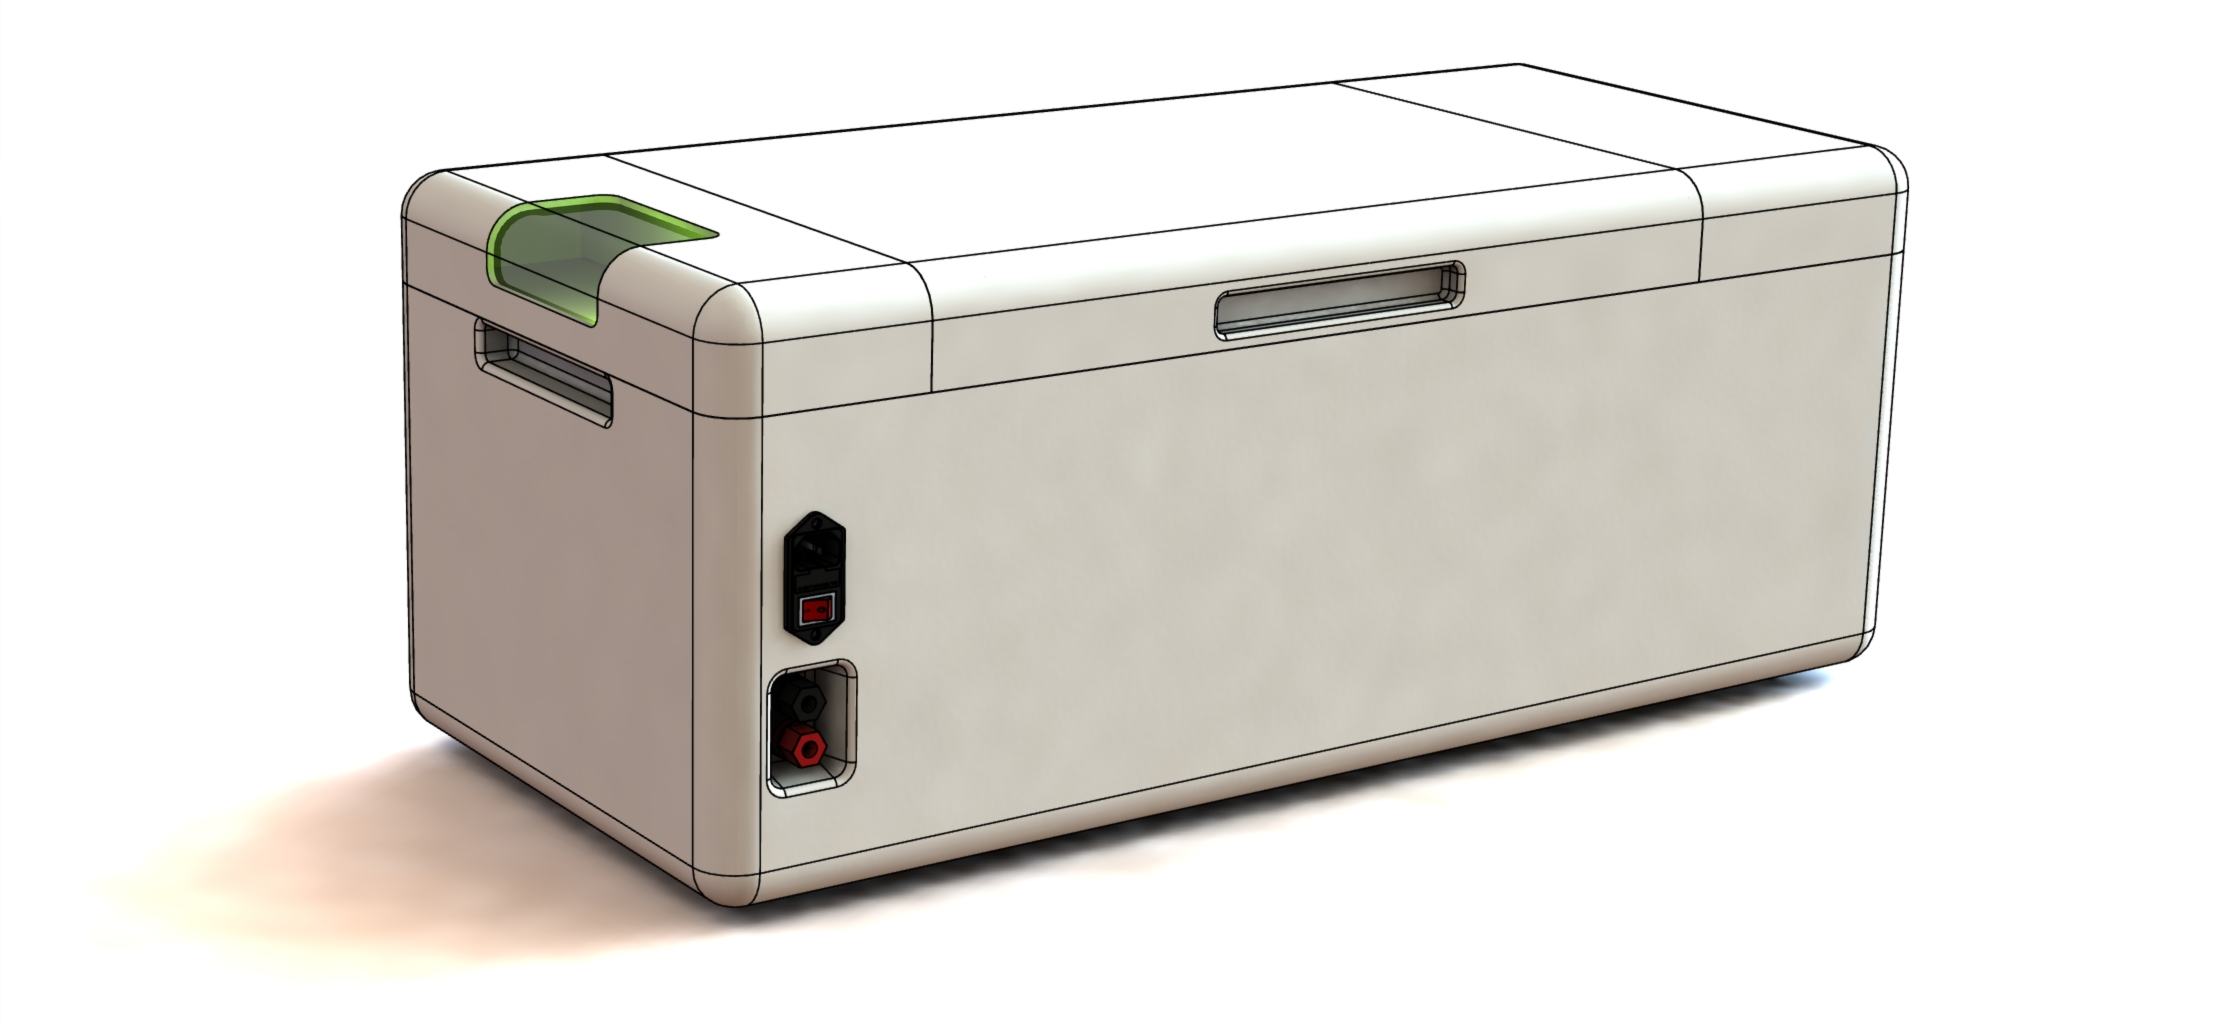
\includegraphics[width=\textwidth]{assets/box_side_render.png}
		\caption[Konzept Rendering]{Konzept Rendering.}
		\label{fig:box side render}
	\end{figure}
	Um einen autarken Betrieb von mindestens \SI{48}{\hour} aufrecht zu erhalten ist ein \SI{74}{\watt\hour} Li-Ion-Akku verbaut. Um im mobilen Einsatz auch bei längeren
	Transportwegen die Kühlung sicher gewährleisten zu können, kann das Produkt von anderen \frq nICE.cube\flq{} parallel versorgt oder durch das mitgelieferte Photovoltaikmodul gespeißt werden.\par\smallskip

	Am besonders energieeffizienten eInk-Display lassen sich jederzeit Parameter wie Innentemperatur, Akkustand Außentemperatur oder geschätze Restlaufzeit\footnote{In Abhängigkeit der
	historischen Außentemperatur und momentanem Akkustand.} kontrollieren. Erreicht der Innenbereich eine vom Benutzer gesetzte kritische Temperatur oder einen niedrigen Akkustand
	wird über sich am Display befindliche Pieper und LEDs wahlweise akustisch und/oder visuell alarmiert.\par\smallskip

	Während die Schalung aus ABS-Kunststoff Komponenten wie Elektronik, Akku und Kompressor vor mechanischen Umwelteinflüssen schützt, sorgt die Schock- und Vibrationsdämpfende Aufhängung
	des Innenbereichs für einen sicheren Transport auch im Gelände.
	\clearpage
	\section{Technische Daten}
		Die technischen Daten des \frq nICE.cube\flq{} im Überblick:\
		\begin{table}[h]
			\centering
			\caption{My awesome Technische Daten}
			\begin{tabular}{@{}p{.3\textwidth}p{.5\textwidth}@{}}
				\toprule
				\textbf{Mechanisch} & \\
				\midrule
				Äußere Dimensionen & 813 x 358 x 314 (LxBxH, Einheiten in \SI{}{\milli\metre})\\
				Nutzvolumen & \SI{16,72}{\litre}\\
				Gesamtgewicht & \SI{22}{\kilo\gram}\\
				\midrule
				\textbf{Elektrisch} & \\
				\midrule
				Kapazität Akku & \SI{72}{\watt\hour}\\
				Versorgungsspannung AC & \SI{230/110}{\volt} \SI{50/60}{\hertz}\\
				Versorgungsspannung DC & \SI{12-24}{\volt}\\
				Kühlleistung & \SI{27,65}{\watt} \cite{Kompressor.datenblatt.Masterflux.20210727}\\

				\bottomrule
			\end{tabular}
			\label{tab:tech daten}
		\end{table}